\documentclass{article}
\usepackage{tikz}
\usetikzlibrary{arrows.meta,positioning,calc,shapes.geometric}
\pagestyle{empty}
\begin{document}
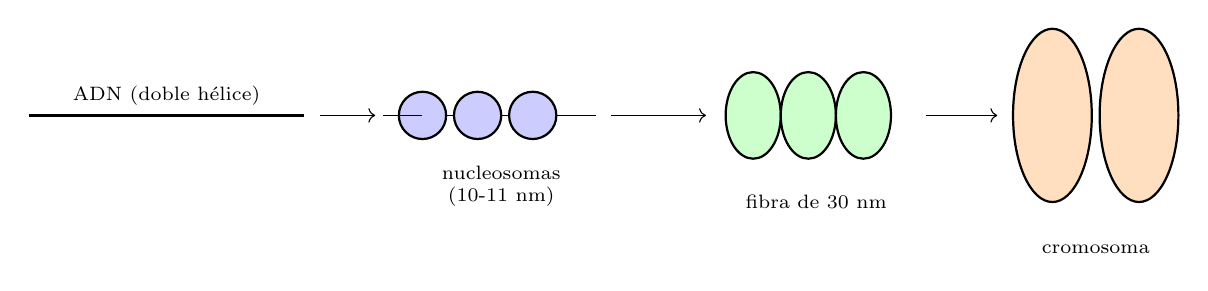
\begin{tikzpicture}
\tikzset{every node/.append style={align=center}}

\draw[thick] (0,0) -- (3.5,0) node[above, midway, font=\scriptsize] {ADN (doble hélice)};
\foreach \x in {5.0,5.7,6.4} {\draw[thick, fill=blue!20] (\x,0) circle (0.3);} \draw (4.5,0) -- (5.0,0); \draw (5.3,0) -- (5.4,0); \draw (6.0,0) -- (6.1,0); \draw (6.7,0) -- (7.2,0);
\node[font=\scriptsize, align=center] at (6,-0.9) {nucleosomas\\ (10-11 nm)};
\foreach \x in {9.2,9.9,10.6} {\draw[thick, fill=green!20] (\x,0) ellipse (0.35 and 0.55);}
\node[font=\scriptsize, align=center] at (10,-1.1) {fibra de 30 nm};
\draw[thick, fill=orange!25] (13,0) ellipse (0.5 and 1.1) ; \draw[thick, fill=orange!25] (14.1,0) ellipse (0.5 and 1.1);
\node[font=\scriptsize, align=center] at (13.55,-1.7) {cromosoma};
\draw[->] (3.7,0) -- (4.4,0); \draw[->] (7.4,0) -- (8.6,0); \draw[->] (11.4,0) -- (12.3,0);

\end{tikzpicture}
\end{document}
